\documentclass{article}
\usepackage[utf8]{inputenc}
\usepackage[T1]{fontenc}
\usepackage{tikz}
\usepackage{amssymb}

\usetikzlibrary{automata, positioning, arrows}

\newcommand{\blank}{\square}

\begin{document}

\begin{center}
\textbf{MT Decisora para $L = \{ a^m b^n \mid m \neq n \}$}
\vspace{1cm}

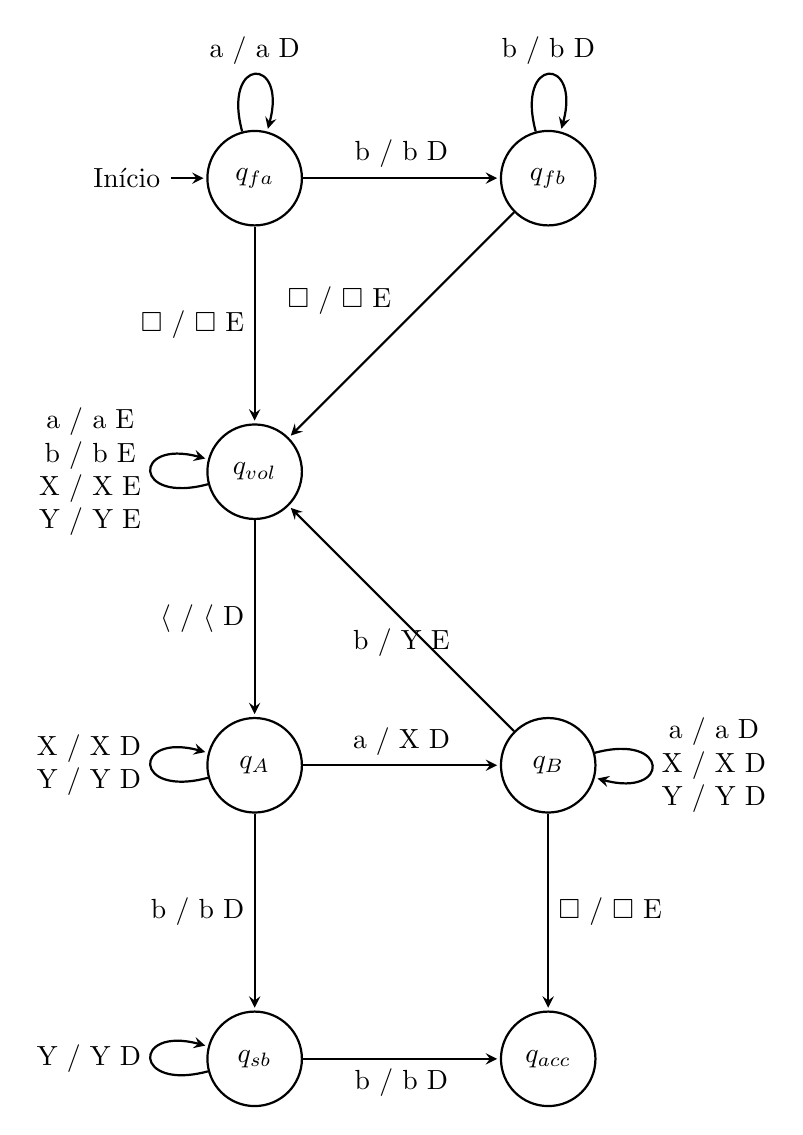
\begin{tikzpicture}[
    ->,
    >=stealth,
    shorten >=1pt,
    auto,
    node distance=2.5cm,
    thick,
    state/.style={circle, draw, minimum size=1.2cm, thick, fill=white},
    accept/.style={double, circle, draw, minimum size=1.2cm, thick, fill=green!10},
    initial text=Início
  ]

  % --- POSICIONAMENTO ---
  \node[state, initial] (qfa) {$q_{fa}$};
  \node[state, right=of qfa] (qfb) {$q_{fb}$};
  \node[state, below=of qfa] (qvol) {$q_{vol}$};
  \node[state, below=of qvol] (qa) {$q_{A}$};
  \node[state, right=of qa] (qb) {$q_{B}$};
  \node[state, below=of qa] (qsb) {$q_{sb}$};
  \node[state, right=of qsb] (acc) {$q_{acc}$};

  % --- TRANSIÇÕES ---

  % 1. Validação
  \path (qfa) edge[loop above] node {a / a D} (qfa)
              edge node {b / b D} (qfb)
              edge node[left] {$\blank$ / $\blank$ E} (qvol);

  \path (qfb) edge[loop above] node {b / b D} (qfb)
              edge node[above left] {$\blank$ / $\blank$ E} (qvol);

  % 2. Retorno (LISTA VERTICAL EXPLÍCITA)
  % Usamos align=center e \\ para quebrar linha
  \path (qvol) edge[loop left] node[align=center] {a / a E \\ b / b E \\ X / X E \\ Y / Y E} (qvol)
               edge node[left] {$\langle$ / $\langle$ D} (qa);

  % 3. Pareamento A
  % Ajustei qA para o mesmo formato vertical para manter consistência
  \path (qa) edge[loop left] node[align=center] {X / X D \\ Y / Y D} (qa)
             edge[right] node[above] {a / X D} (qb)
             edge node[left] {b / b D} (qsb);

  % 4. Pareamento B (LISTA VERTICAL EXPLÍCITA)
  \path (qb) edge[loop right] node[align=center] {a / a D \\ X / X D \\ Y / Y D} (qb)
             edge[above left] node[below] {b / Y E} (qvol)
             edge[below] node[right] {$\blank$ / $\blank$ E} (acc);

  % 5. Sobra B
  \path (qsb) edge[loop left] node {Y / Y D} (qsb)
              edge node[below] {b / b D} (acc);

\end{tikzpicture}
\end{center}

\end{document}